\documentclass{article}
\usepackage{graphicx}
\usepackage{amsmath}
\usepackage{amssymb}
\usepackage{listings}
\usepackage[margin=1in]{geometry}
\usepackage{xcolor}
\usepackage{enumitem}
\usepackage{pgfplots}
\usepackage{tikz}
\usetikzlibrary{shapes, arrows, positioning, calc, backgrounds}
\usepackage{tcolorbox}
\usepackage{bm}

% Define colors for syntax highlighting
\definecolor{codegreen}{rgb}{0,0.6,0}
\definecolor{codegray}{rgb}{0.5,0.5,0.5}
\definecolor{codepurple}{rgb}{0.58,0,0.82}
\definecolor{backcolour}{rgb}{0.95,0.95,0.92}

% Python style for highlighting
\lstdefinestyle{pythonstyle}{
    backgroundcolor=\color{backcolour},   
    commentstyle=\color{codegreen},
    keywordstyle=\color{magenta},
    numberstyle=\tiny\color{codegray},
    stringstyle=\color{codepurple},
    basicstyle=\ttfamily\footnotesize,
    breakatwhitespace=false,         
    breaklines=true,                 
    captionpos=b,                    
    keepspaces=true,                 
    numbers=left,                    
    numbersep=5pt,                  
    showspaces=false,                
    showstringspaces=false,
    showtabs=false,                  
    tabsize=2
}
\lstset{style=pythonstyle}

\title{Lecture: Breaking the Seq2Seq Bottleneck\\
\large Cross-Attention via Learned Kernel Regression}
\author{Deep Learning Class}
\date{\today}

\begin{document}
\maketitle

\begin{tcolorbox}[colback=blue!5!white, colframe=blue!75!black, title=Lecture Arc]
Today's journey:
\begin{enumerate}
    \item The seq2seq bottleneck problem (with concrete examples)
    \item Solution: maintain a full memory bank (the human translator analogy)
    \item Kernel regression as the conceptual bridge
    \item Attention as learned data pooling
    \item Decoder cross-attention mechanisms (additive $\rightarrow$ dot-product evolution)
    \item Practical considerations: scaling, masking, batching
    \item Multi-head attention for multiple perspectives
    \item The leap to self-attention (next lecture preview)
\end{enumerate}
\end{tcolorbox}

\section{The Seq2Seq Bottleneck Problem}

Last lecture, we built sequence-to-sequence models for tasks like machine translation. The architecture had a beautiful simplicity: an RNN encoder processes the source sequence and produces a single context vector $c$, which the decoder RNN then uses to generate the target sequence.

\begin{figure}[h]
\centering
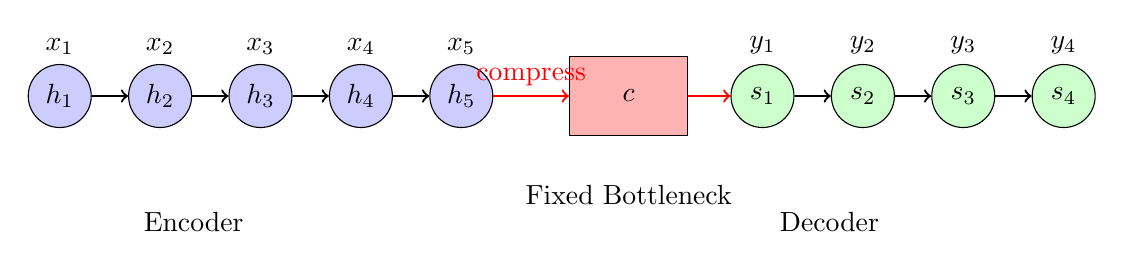
\begin{tikzpicture}[scale=0.85]
    % Encoder
    \foreach \i in {1,...,5} {
        \node[draw, circle, minimum size=0.8cm, fill=blue!20] (enc\i) at (\i*1.5, 0) {$h_\i$};
        \node[above] at (enc\i.north) {$x_\i$};
    }
    
    % Connections in encoder
    \foreach \i in {1,...,4} {
        \pgfmathtruncatemacro{\j}{\i+1}
        \draw[->, thick] (enc\i) -- (enc\j);
    }
    
    % The bottleneck
    \node[draw, rectangle, minimum width=1.5cm, minimum height=1cm, fill=red!30] (bottleneck) at (10, 0) {$c$};
    \draw[->, thick, red] (enc5) -- (bottleneck) node[midway, above] {compress};
    
    % Decoder
    \foreach \i in {1,...,4} {
        \node[draw, circle, minimum size=0.8cm, fill=green!20] (dec\i) at (10.5+\i*1.5, 0) {$s_\i$};
        \node[above] at (dec\i.north) {$y_\i$};
    }
    
    % Connections in decoder
    \draw[->, thick, red] (bottleneck) -- (dec1);
    \foreach \i in {1,...,3} {
        \pgfmathtruncatemacro{\j}{\i+1}
        \draw[->, thick] (dec\i) -- (dec\j);
    }
    
    \node[below=0.5cm] at (3.5, -1) {Encoder};
    \node[below=0.5cm] at (bottleneck.south) {Fixed Bottleneck};
    \node[below=0.5cm] at (13, -1) {Decoder};
\end{tikzpicture}
\caption{Vanilla seq2seq: Everything must flow through a single fixed-size vector $c$}
\end{figure}

\subsection{A Concrete Example: Why the Bottleneck Hurts}

Consider translating this French sentence to English:

\begin{center}
\textit{``Je ne suis pas le chat noir''} $\rightarrow$ \textit{``I am not the black cat''}
\end{center}

This seemingly simple sentence reveals the bottleneck problem:

\begin{itemize}
    \item \textbf{Word order differs}: French uses double negation (``ne...pas''), which English doesn't have
    \item \textbf{Adjective placement}: French puts adjectives after nouns (``chat noir''), English reverses this (``black cat'')
    \item \textbf{Distance matters}: The word ``ne'' (position 2) and ``pas'' (position 4) must be coordinated, but they're separated
\end{itemize}

The encoder must somehow compress all this structural information---word positions, grammatical dependencies, semantic roles---into a single fixed-dimensional vector. When the sentence gets longer, this becomes impossible.

\begin{tcolorbox}[colback=red!5!white, colframe=red!50!black, title=The Empirical Evidence]
Bahdanau et al. (2014) and Sutskever et al. (2014) showed that translation quality (measured by BLEU score) degrades significantly for sentences longer than 30-40 tokens. The single context vector $c$ becomes a severe information bottleneck. In some early large-scale models, the softmax operation over large vocabularies also became a computational bottleneck, but the conceptual bottleneck---compressing long sequences---was the fundamental problem.
\end{tcolorbox}

\begin{tcolorbox}[colback=orange!5!white, colframe=orange!75!black, title=Backlog: Costs of Recurrence]
Beyond the information bottleneck, the RNN architecture used in vanilla seq2seq has other fundamental limitations:
\begin{itemize}
    \item \textbf{Sequential Computation (The Parallelization Problem)}: RNNs must process sequences token by token. $h_t$ cannot be computed before $h_{t-1}$. This prevents parallelization on modern hardware (GPUs/TPUs), making training slow and limiting scalability.
    \item \textbf{Gradient Propagation}: Although LSTMs and GRUs mitigate vanishing/exploding gradients, propagating information through many time steps remains challenging, making it difficult to reliably learn very long-range dependencies.
\end{itemize}
While today's focus is solving the information bottleneck, keep these computational constraints in mind---they will motivate the radical architectural shift we discuss next lecture.
\end{tcolorbox}

\subsection{Why This Matters}

The bottleneck is especially severe for:
\begin{itemize}
    \item Long sentences with complex syntactic structure
    \item Languages with very different word orders
    \item Tasks requiring fine-grained alignment (e.g., word-level translation, summarization)
    \item Any scenario where different parts of the output depend on different parts of the input
\end{itemize}

\section{The Key Insight: A Memory Bank, Not a Single Vector}

How do humans solve this problem? A human translator:
\begin{enumerate}
    \item Reads the entire source sentence (encoding phase)
    \item Keeps the \textit{entire} source in working memory (not just a summary!)
    \item When generating each target word, looks back at relevant parts of the source
    \item Dynamically shifts attention as the translation progresses
\end{enumerate}

This suggests a simple: \textbf{Why throw away all those intermediate encoder states?}

In the vanilla model, we compute hidden states $h_1, h_2, \ldots, h_T$ in the encoder, but only use the final state $h_T$. What if we kept them all?

\begin{tcolorbox}[colback=green!5!white, colframe=green!50!black, title=Dynamic Memory Access]
Transform the latent space from a single vector into a \textbf{sequence of memory slots}:
\begin{itemize}
    \item Old: $c \in \mathbb{R}^d$ (one summary vector)
    \item New: $\{h_1, h_2, \ldots, h_T\}$ where each $h_i \in \mathbb{R}^d$ (full memory bank)
\end{itemize}

The decoder can then \textbf{selectively access} whichever parts of this memory bank are relevant at each decoding step. This is \textit{dynamic lookup}, not fixed compression.
\end{tcolorbox}

\subsection{The Attention-Augmented Architecture}

It is crucial to understand the architectural context. We are not yet replacing the Seq2Seq model; we are \textbf{augmenting} it. The encoder and the decoder are still Recurrent Neural Networks (e.g., LSTMs or GRUs).

\begin{itemize}
    \item The \textbf{Encoder RNN} still processes the input sequentially to compute the hidden states $\{h_i\}$.
    \item The \textbf{Decoder RNN} still generates the output sequentially, maintaining its own state $s_t$.
    \item \textbf{Attention} acts as a bridge, allowing the decoder RNN to access the full memory bank $\{h_i\}$ when calculating the dynamic context $c_t$.
\end{itemize}

\begin{tcolorbox}[colback=blue!5!white, colframe=blue!75!black, title=Terminology: Cross-Attention]
The mechanism we are describing today is specifically called \textbf{Cross-Attention}.

It is called ``cross'' because the attention mechanism bridges two \textit{different} sequences: the decoder state (the query) attends ``across'' to the encoder memory (the keys and values). We will contrast this next lecture with \textbf{Self-Attention}, where a single sequence attends to itself.
\end{tcolorbox}

\begin{figure}[h]
\centering
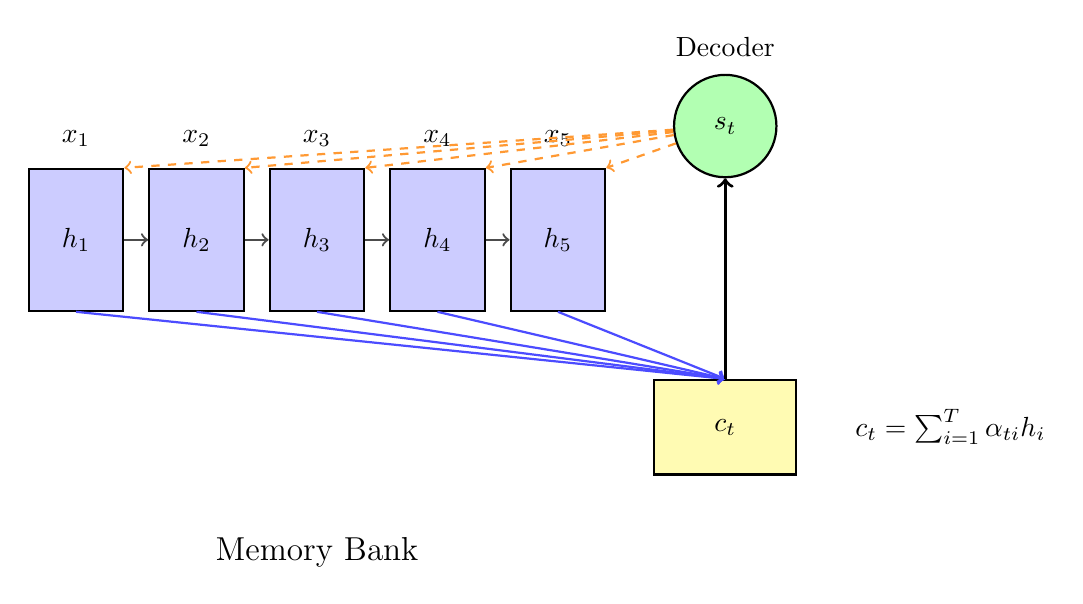
\begin{tikzpicture}[scale=0.85]
    % Encoder states (memory bank)
    \foreach \i in {1,...,5} {
        \node[draw, rectangle, minimum width=1.2cm, minimum height=1.8cm, 
              fill=blue!20, line width=0.8pt] (mem\i) at (\i*1.8, 0) {};
        \node at (\i*1.8, 0) {$h_\i$};
        \node[above=0.15cm] at (mem\i.north) {$x_\i$};
    }
    
    % Forward recurrent connections
    \foreach \i in {1,...,4} {
        \pgfmathtruncatemacro{\j}{\i+1}
        \draw[->, thick, black!70] (mem\i.east) -- (mem\j.west);
    }
    
    % Current decoder state
    \node[draw, circle, minimum size=1.3cm, fill=green!30, line width=0.8pt] 
        (decoder) at (11.5, 1.7) {$s_t$};
    \node[above=0.1cm] at (decoder.north) {Decoder};
    
    % Attention query connections (decoder to encoder states)
    \foreach \i in {1,...,5} {
        \draw[->, dashed, orange!80, thick] (decoder) -- (mem\i.north east);
    }
    
    % Context vector
    \node[draw, rectangle, minimum width=1.8cm, minimum height=1.2cm, 
          fill=yellow!30, line width=0.8pt] (context) at (11.5, -2.8) {$c_t$};
    
    % Weighted sum arrows (encoder states to context)
    \foreach \i in {1,...,5} {
        \draw[->, blue!70, thick] (mem\i.south) -- (context.north);
    }
    
    % Connection from context to decoder
    \draw[->, very thick, black] (context.north) -- (decoder.south);
    
    % Labels
    \node[below=0.25cm, font=\large] at (5.4, -4) {Memory Bank};
    \node[right, align=left] at (13.3, -2.8) 
        {$c_t = \sum_{i=1}^{T} \alpha_{ti} h_i$};
\end{tikzpicture}
\caption{Attention mechanism: The decoder dynamically accesses all encoder states}
\end{figure}

\subsection{How Dynamic Access Works}

At each decoding step $t$, the decoder:
\begin{enumerate}
    \item Examines its current state $s_t$ (``What have I generated so far?'')
    \item Queries the encoder memory bank $\{h_1, \ldots, h_T\}$ (``What information is available?'')
    \item Computes how relevant each $h_i$ is to generating the next token (``Where should I focus?'')
    \item Creates a custom context vector $c_t$ as a weighted combination (``Let me aggregate the relevant information'')
\end{enumerate}


The crucial difference: $c_t$ is \textbf{dynamic}---it changes at each step based on what the decoder needs. When translating ``chat noir'' to ``black cat'', the decoder can attend to ``noir'' when generating ``black'', then attend to ``chat'' when generating ``cat''.

\begin{tcolorbox}[colback=gray!5!white, colframe=black!50!black, title=A Note on Sequence Order]
Observe that the attention mechanism itself, as described, is a ``bag of vectors'' operation. The context vector $c_t = \sum \alpha_{ti} h_i$ is a weighted sum, which is permutation-invariant (shuffling the order of $h_i$ does not change the result if the weights are adjusted accordingly). So how does the model know the order of the input words?

In this architecture, the sequential information is still handled by the underlying RNNs. The encoder states $\{h_i\}$ are generated recurrently, embedding positional context within them.

This reliance on recurrence is important. Next lecture, when we remove the RNNs, we will need a new mechanism to inject positional information.
\end{tcolorbox}

\section{Kernel Regression: The Conceptual Bridge}

Now we face a key question: \textit{How do we implement this dynamic lookup mechanism?} We need the decoder to query the memory bank and retrieve a weighted combination of the encoder states. Crucially, this lookup must be \textbf{differentiable} so we can train the entire system end-to-end. We need a ``soft'' way to access memory, rather than a hard lookup (like indexing an array).
It turns out this problem of differentiable, soft data retrieval was solved 60 years ago in statistics!

Given observed data points $\{(x_i, y_i)\}_{i=1}^n$, where $x_i \in \mathbb{R}^d$ are coordinates and $y_i \in \mathbb{R}$ are values. For a new query point $q$, we want to predict its value $f(q)$.
The Nadaraya-Watson (NW) estimator (1964) provides a solution using a fixed similarity function:
The prediction is a \textbf{weighted average} of all observed values:

\begin{equation}
\hat{f}(q) = \sum_{i=1}^{n} w_i(q) \cdot y_i
\end{equation}

The weights are defined using a \textbf{kernel function} $K(\cdot, \cdot)$ that measures similarity:

\begin{equation}
w_i(q) = \frac{K(q, x_i)}{\sum_{j=1}^{n} K(q, x_j)}
\end{equation}

\begin{center}
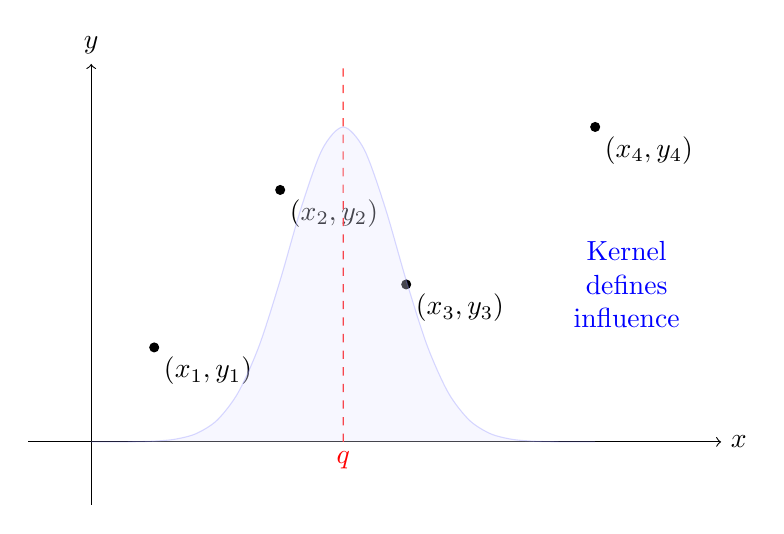
\begin{tikzpicture}[scale=0.8]
    % Axes
    \draw[->] (-1,0) -- (10,0) node[right] {$x$};
    \draw[->] (0,-1) -- (0,6) node[above] {$y$};

    % Data points
    \coordinate (P1) at (1, 1.5); 
    \coordinate (P2) at (3, 4);
    \coordinate (P3) at (5, 2.5); 
    \coordinate (P4) at (8, 5);

    \draw[fill=black] (P1) circle (2pt) node[below right] {$(x_1, y_1)$};
    \draw[fill=black] (P2) circle (2pt) node[below right] {$(x_2, y_2)$};
    \draw[fill=black] (P3) circle (2pt) node[below right] {$(x_3, y_3)$};
    \draw[fill=black] (P4) circle (2pt) node[below right] {$(x_4, y_4)$};

    % Query point
    \coordinate (Q) at (4,0);
    \draw[red, dashed] (Q) -- (4, 6);
    \node[below, red] at (Q) {$q$};

    % Kernel visualization
    \draw[blue!50, domain=0:8, smooth, variable=\x, opacity=0.3, fill=blue!10] 
        plot ({\x}, {5*exp(-((\x-4)^2)/1.5)});

    \node[align=center, blue] at (8.5, 2.5) {Kernel\\defines\\influence};
\end{tikzpicture}
\end{center}

The Gaussian (Radial Basis Function) kernel is widely used:

\begin{equation}
K(q, x) = \exp\left(-\frac{1}{2h^2}\|q - x\|^2\right)
\end{equation}

where $h$ is the bandwidth parameter. Points closer to $q$ (smaller $\|q - x\|$) receive higher weights. This is exactly the kind of ``pay more attention to similar things'' behavior we want.

The main limitation of NW estimator: the kernel $K(q, x)$ is fixed and hand-crafted. We're about to see how to make it learnable.

\section{From Kernel Regression to Attention}
We can rewrite the prediction problem in a generalized form:
\begin{equation}
f(q) = \sum_{i=1}^{n} \alpha(q, x_i) \cdot y_i
\end{equation}
This is \textbf{attention pooling}: we aggregate/pool the observed values $y_i$, where the pooling weights $\alpha(q, x_i)$ depend on the similarity between the query $q$ and each coordinate $x_i$.

Attention mechanisms in deep learning are  learnable forms of this data pooling operation.
Let us now make the connection explicit. We reinterpret kernel regression using the language of attention mechanisms:

\begin{center}
\begin{tabular}{|l|l|l|}
\hline
\textbf{Concept} & \textbf{Kernel Regression} & \textbf{Attention in Seq2Seq} \\
\hline
\textbf{Query} & Query point $q$ & Decoder state $s_t$ \\
 & (Where to predict?) & (What do I need to output now?) \\
\hline
\textbf{Keys} & Coordinates $\{x_i\}$ & Encoder states $\{h_i\}$ \\
 & (Where is data located?) & (What information is available?) \\
\hline
\textbf{Values} & Observations $\{y_i\}$ & Encoder states $\{h_i\}$ \\
 & (What to aggregate?) & (Content to retrieve) \\
\hline
\textbf{Weights} & $w_i = \frac{K(q, x_i)}{\sum_j K(q, x_j)}$ & $\alpha_{ti} = \frac{\exp(a(s_t, h_i))}{\sum_j \exp(a(s_t, h_j))}$ \\
 & (How much to weight each value?) & (How much to focus on each encoder state?) \\
\hline
\textbf{Output} & $\hat{f}(q) = \sum_i w_i y_i$ & $c_t = \sum_i \alpha_{ti} h_i$ \\
 & (Predicted value) & (Context vector) \\
\hline
\end{tabular}
\end{center}


\paragraph{The General Attention Formula:}
The attention mechanism computes:
\begin{equation}
\text{Attention}(q, K, V) = \sum_{i=1}^{T} \alpha_i(q) \cdot v_i
\end{equation}

where the attention weights are computed using softmax over a scoring function $a(q, k_i)$:

\begin{equation}
\alpha_i(q) = \frac{\exp(a(q, k_i))}{\sum_{j=1}^{T} \exp(a(q, k_j))} = \text{softmax}(a(q, K))_i
\end{equation}

\subsection{Connection to Kernels}

If we define the kernel as $K(q, k_i) = \exp(a(q, k_i))$, then attention weights are exactly the Nadaraya-Watson weights. This reveals:

\begin{equation}
a(q, k_i) = \log K(q, k_i)
\end{equation}

For the Gaussian kernel:
\begin{equation}
a(q, k_i) = -\frac{1}{2h^2}\|q - k_i\|^2
\end{equation}

Working in log-space (with scores $a$) is computationally convenient: we can use gradient descent to optimize $a(\cdot, \cdot)$ directly. The exponential in softmax converts these learned scores back to proper probability-like weights.

\section{Learning the Attention Mechanism: An Evolution}

Now we arrive at the heart of modern attention: making the similarity function learnable. This evolution happened in two major steps.

\begin{center}
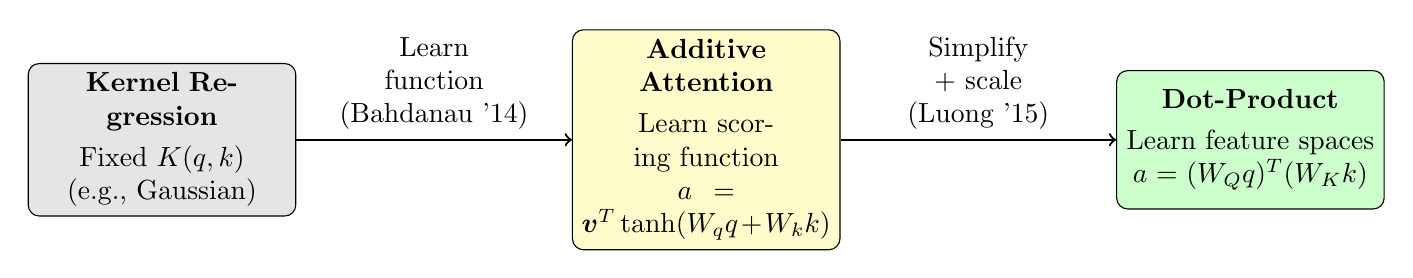
\begin{tikzpicture}[node distance=3.5cm, auto]
    \tikzstyle{block} = [rectangle, draw, text width=9em, text centered, 
                         rounded corners, minimum height=5em]

    \node [block, fill=gray!20] (kr) {
        \textbf{Kernel Regression}\\[0.3em]
        Fixed $K(q, k)$\\
        (e.g., Gaussian)
    };
    \node [block, fill=yellow!20, right=of kr] (add) {
        \textbf{Additive Attention}\\[0.3em]
        Learn scoring function\\
        $a = \bm{v}^T \tanh(W_q q + W_k k)$
    };
    \node [block, fill=green!20, right=of add] (dot) {
        \textbf{Dot-Product}\\[0.3em]
        Learn feature spaces\\
        $a = (W_Q q)^T (W_K k)$
    };

    \draw[->, thick] (kr) -- node[align=center, above] {Learn\\function\\(Bahdanau '14)} (add);
    \draw[->, thick] (add) -- node[align=center, above] {Simplify\\+ scale\\(Luong '15)} (dot);
\end{tikzpicture}
\end{center}
where each step increases \textit{learnability} while improving \textit{efficiency}:
\begin{enumerate}
    \item \textbf{Fixed kernels} (NW regression): Hand-crafted similarity using Euclidean distance
    \item \textbf{Additive attention} (Bahdanau 2014): Learn a neural network to compute similarity
    \item \textbf{Dot-product attention} (Luong 2015, Vaswani 2017): Learn projection matrices to create feature spaces where dot products measure similarity
\end{enumerate}


\section{Additive Attention: Learning the Scoring Function}

\paragraph{The Original Solution (Bahdanau et al., 2014).}
The key idea is to \emph{learn} what ``similarity'' should mean for the task (kernel) via a tiny neural network (an MLP with one hidden layer and $\tanh$) scores how well a decoder state $\bm{s}_t$ (the \emph{query}) should attend to an encoder state $\bm{h}_i$ (the \emph{key/value}).

\begin{equation}
\label{eq:bahdanau}
e_{t,i}
\;=\;
a(\bm{s}_t,\bm{h}_i)
\;=\;
\bm{v}_a^{\!\top}\,
\tanh\!\big(
W_q\,\bm{s}_t \;+\; W_k\,\bm{h}_i \;+\; \bm{b}
\big),
\qquad
\begin{aligned}
&W_q \in \mathbb{R}^{d_h\times d_{\text{dec}}},\\
&W_k \in \mathbb{R}^{d_h\times d_{\text{enc}}},\\
&\bm{v}_a,\bm{b}\in\mathbb{R}^{d_h}.
\end{aligned}
\end{equation}

\noindent The attention weights and context are then
\begin{equation}
\alpha_{t,i}
=\frac{\exp(e_{t,i})}{\sum_{j}\exp(e_{t,j})},
\qquad
\bm{c}_t=\sum_{i}\alpha_{t,i}\,\bm{h}_i,
\end{equation}
and the decoder uses \((\bm{s}_t,\bm{c}_t)\) to predict the next token.

\paragraph{What do \(W_q\), \(W_k\), and \(\bm{v}_a\) \emph{do}? (Interpretation)}
\begin{itemize}
  \item \(\boxed{W_q}\) and \(\boxed{W_k}\) are \textbf{learned projections} that map queries (\(\bm{s}_t\)) and keys (\(\bm{h}_i\)) into a \emph{common alignment space} of dimension \(d_h\).
  \begin{itemize}
    \item This lets the model \(\rightarrow\) (i) compare objects of \emph{different} sizes (\(d_{\text{dec}}\neq d_{\text{enc}}\)), (ii) learn feature re-weightings and cross-dimensional mixes before comparing.
    \item Pedagogical picture: they linearly transform both \(\bm{s}_t\) and
    \(\bm{h}_i\) so that useful components line up for comparison. A learned linear
    map may rotate, scale, shear, or project.
  \end{itemize}
  \item \(\boxed{\tanh(\cdot)}\) injects a \textbf{nonlinear interaction} between the projected vectors, enabling richer, non-bilinear matching (beyond a cosine/dot).
  \item \(\boxed{\bm{v}_a}\) is a \textbf{feature selector} in alignment space: after computing the \(d_h\)-dimensional match features, the scalar score \(e_{t,i}\) is the projection onto direction \(\bm{v}_a\).
  \begin{itemize}
    \item View it as ``which alignment features actually matter?”—\(\bm{v}_a\) assigns positive/negative importance to each hidden feature produced by \(\tanh(W_q\bm{s}_t+W_k\bm{h}_i+\bm{b})\).
    \item Equivalently, \eqref{eq:bahdanau} is a 1-hidden-layer MLP with shared parameters over all pairs \((t,i)\): \(\Theta=\{W_q,W_k,\bm{b},\bm{v}_a,c\}\) applied to every pair \((t,i)\). The sharing is across all positions \(t\) and \(i\).

  \end{itemize}
\end{itemize}








\paragraph{Why it worked (and what it fixed).}
\begin{itemize}
  \item \textbf{Removes the bottleneck.} The decoder no longer compresses the entire source into a single vector; it \emph{adapts} a context \(\bm{c}_t\) at each step.
  \item \textbf{Soft alignment.} The weights \(\alpha_{t,i}\) behave like differentiable alignments from target positions \(t\) to source positions \(i\).
  \item \textbf{Historical positioning.} Additive attention (Bahdanau et al., 2014/15) significantly advanced the original seq2seq LSTM breakthrough (Sutskever et al., 2014).
\end{itemize}



\begin{tcolorbox}[colback=yellow!5!white, colframe=orange!50!black, title=The Hardware Insight: Vectorized view and computational footprint]
Modern accelerators (GPUs/TPUs) are highly optimized for dense matrix multiplication (BLAS operations). Additive attention requires complex, fused operations. If we can reformulate attention purely as matrix multiplication, we can achieve massive speedups and scalability. This efficiency is critical for training large models.

Let \(T\) be target length and \(N\) source length. Define
\(\;A = [A_{t,:}]_{t=1}^T = [W_q\bm{s}_t]_{t=1}^T \in \mathbb{R}^{T\times d_h}\)
and
\(\;B = [B_{i,:}]_{i=1}^N = [W_k\bm{h}_i]_{i=1}^N \in \mathbb{R}^{N\times d_h}\).
Then the pairwise hidden features are
\[
H_{t,i,:} \;=\; \tanh\!\big(A_{t,:} + B_{i,:} + \bm{b}\big)\;\in\;\mathbb{R}^{d_h},
\quad
e_{t,i} \;=\; \bm{v}_a^{\!\top} H_{t,i,:}.
\]
Computing \(\{e_{t,i}\}\) naively materializes an \(\mathcal{O}(TN d_h)\) tensor and performs elementwise nonlinearity + reduction. This pattern is \textbf{broadcast-heavy and memory-bound}: it underutilizes GPU/TPU tensor-core units, which are optimized for large dense \(\texttt{GEMM}\)s (BLAS \(\mathtt{gemm}\)).\\
\textbf{Modern accelerators and ``make it matmul'':}
GPUs/TPUs hit peak FLOPs on big matrix multiplies. Additive attention’s core operation,
\(\tanh(A_{t,:}+B_{i,:})\),
is \emph{not separable} and does \emph{not} collapse into a small number of GEMMs; it needs outer-sums/broadcasts, elementwise \(\tanh\), then a reduction by \(\bm{v}_a\).
We really wish to replace this operation with GEMM-friendly operations (The answer: use the dot product, but learn the right feature spaces first!).
\end{tcolorbox}



\paragraph{From additive to GEMM-friendly variants (for scale).}
\begin{itemize}
  \item \textbf{Bilinear/general attention:} Replace \(\tanh\) with identity and fold \(\bm{v}_a\) into a matrix \(W\):
  \(e_{t,i}=\bm{s}_t^{\!\top}W\bm{h}_i\).
  With a factorization \(W=U^{\top}V\), you get two projections \((U\bm{s}_t, V\bm{h}_i)\) plus a dot product \(\Rightarrow\) GEMMs.
  \item \textbf{Scaled dot-product (Transformer default):} \(e_{t,i}=\bm{q}_t^{\!\top}\bm{k}_i/\sqrt{d}\), keeping the hot path as GEMMs with fused softmax/masking (Flash-style kernels).
  \item \textbf{Kernel/linear attention:} Approximate \(\exp(\bm{q}^{\top}\bm{k})\approx \phi(\bm{q})^{\top}\phi(\bm{k})\), yielding
  \(\operatorname{Attn}(Q,K,V)\approx \phi(Q)\big(\phi(K)^{\top}V\big)\) with two GEMMs and no \(TN\) matrix materialization.
\end{itemize}






\subsection{Implementation}

\begin{lstlisting}[language=Python, caption=Additive Attention Implementation]
import torch
import torch.nn as nn
import torch.nn.functional as F

class AdditiveAttention(nn.Module):
    def __init__(self, key_size, query_size, hidden_size, dropout=0.0):
        super().__init__()
        self.W_k = nn.Linear(key_size, hidden_size, bias=False)
        self.W_q = nn.Linear(query_size, hidden_size, bias=False)
        self.w_v = nn.Linear(hidden_size, 1, bias=False)
        self.dropout = nn.Dropout(dropout)
        
    def forward(self, queries, keys, values, valid_lens=None):
        """
        queries: (batch_size, num_queries, query_size)
        keys: (batch_size, num_keys, key_size)
        values: (batch_size, num_keys, value_size)
        valid_lens: (batch_size,) or (batch_size, num_queries)
        """
        # Project queries and keys
        queries = self.W_q(queries)  # (b, num_q, hidden)
        keys = self.W_k(keys)         # (b, num_k, hidden)
        
        # Broadcasting: (b, num_q, 1, h) + (b, 1, num_k, h)
        # Result: (b, num_q, num_k, h)
        features = torch.tanh(
            queries.unsqueeze(2) + keys.unsqueeze(1)
        )
        
        # Compute scores: (b, num_q, num_k, h) -> (b, num_q, num_k)
        scores = self.w_v(features).squeeze(-1)
        
        # Apply masked softmax
        attention_weights = masked_softmax(scores, valid_lens)
        
        # Apply dropout and compute weighted sum
        return torch.bmm(self.dropout(attention_weights), values)
\end{lstlisting}

\section{Dot-Product Attention: Learning the Feature Space}
While additive attention works well, it has a computational cost: we must run a small neural network (the MLP inside the additive function) for every query-key pair. For long sequences, this becomes expensive.

The next evolution asks: \textit{Can we use a simpler, more efficient similarity function?}




\subsection{Two Complementary Views}

There are two beautiful ways to understand how we get from distance-based kernels to dot products.


\subsubsection{View 1: The Kernel Trick (Feature Space Perspective)}

For a symmetric positive-semidefinite kernel satisfying the usual regularity
conditions, Mercer's theorem gives an inner-product representation in a feature
space:

\begin{equation}
K(q, k) = \langle \phi(q), \phi(k) \rangle_{\mathcal{H}}
\end{equation}

where $\phi: \mathbb{R}^d \rightarrow \mathcal{H}$ maps inputs to a (possibly infinite-dimensional) Hilbert space.

\begin{tcolorbox}[colback=green!5!white, colframe=green!50!black, title=Core Insight: Explicit vs. Implicit Feature Maps]
\begin{itemize}
    \item \textbf{Classical kernels}: Use fixed, implicit feature maps
    \begin{equation}
    K(q, k) = \langle \phi(q), \phi(k) \rangle \quad \text{($\phi$ is implicit and fixed)}
    \end{equation}
    
    \item \textbf{Attention scores}: Use two learned, explicit projections
    \begin{align}
    \phi_Q(q) &= W_Q q \quad \text{(Query projection)} \\
    \phi_K(k) &= W_K k \quad \text{(Key projection)} \\
    a(q, k) &= \langle \phi_Q(q), \phi_K(k) \rangle = (W_Q q)^T (W_K k)
    \end{align}
\end{itemize}

This is a useful analogy, not a claim that every attention score is a Mercer kernel.
When $W_Q\ne W_K$, the score can be asymmetric and need not be positive
semidefinite. Attention \textbf{learns} this task-specific bilinear similarity from
data rather than requiring the classical kernel conditions.
\end{tcolorbox}

Why is this powerful?
\begin{enumerate}
    \item \textbf{Asymmetry}: Separate $W_Q$ and $W_K$ allow different projections. The query asks ``what am I looking for?'' while the key answers ``what do I offer?''
    \item \textbf{Finite dimensions}: Unlike infinite-dimensional kernel spaces, we use tractable projections
    \item \textbf{Task adaptation}: $W_Q, W_K$ adapt through backpropagation, discovering the most useful notion of similarity
    \item \textbf{Computational efficiency}: The formulation reduces to highly optimized matrix multiplications (GEMMs), which map well to GPU/TPU hardware
\end{enumerate}

\paragraph{The Critical Question: Where Does Non-linearity Come From?}

The projections $W_Q$ and $W_K$ are linear, but attention as a whole is not merely a
stack of linear maps: the scores pass through a softmax and create input-dependent
mixing weights. Surrounding recurrent cells, normalization, gating, and feed-forward
networks add further nonlinear transformations.

The answer is that the attention mechanism does not operate in isolation; it relies on the \textit{surrounding architecture} to provide the non-linearity.

\begin{itemize}
    \item In the \textbf{RNN Seq2Seq} model (our current context), the inputs ($s_t$ and $h_i$) are outputs of deep LSTMs or GRUs, which have already performed complex, nonlinear transformations on the sequence.
    \item In the \textbf{Transformer} architecture (next lecture), nonlinear behavior
    comes from the attention softmax and from the surrounding block, including the
    positionwise feed-forward network (FFN), normalization, and any gates or activations.
\end{itemize}

\begin{tcolorbox}[colback=blue!5!white, colframe=blue!75!black, title=A Kernel Analogy: The Role of the FFN]

In the ``kernel trick'' analogy, attention compares nonlinearly encoded token
representations with a learned bilinear score. The \textbf{positionwise FFN} is one
important source of tokenwise nonlinear features; it is not the only nonlinearity in
the block. The query/key matrices are general linear projections---not necessarily
rotations---and their asymmetric score is best called a task-adapted similarity.

Let $z_i^{(\ell)}\in\mathbb{R}^{d_{\mathrm{model}}}$ be the token representation at layer $\ell$.
A Transformer block can be abstracted as
\begin{align}
\tilde{z}_i^{(\ell)} &= z_i^{(\ell)} + \mathrm{MHA}\big(\mathrm{LN}(z^{(\ell)})\big)_i, \\
z_i^{(\ell+1)} &= \tilde{z}_i^{(\ell)} + \underbrace{\mathrm{FFN}\big(\mathrm{LN}(\tilde{z}_i^{(\ell)})\big)}_{\text{tokenwise, nonlinear}}.
\end{align}
A standard FFN is a two-layer MLP
\begin{equation}
\mathrm{FFN}(x) = W_2\,\sigma(W_1 x + b_1) + b_2,
\qquad
W_1\in\mathbb{R}^{d_{\mathrm{hid}}\times d_{\mathrm{model}}}, W_2\in\mathbb{R}^{d_{\mathrm{model}}\times d_{\mathrm{hid}}},
\end{equation}
or a gated variant (e.g., SwiGLU)
\begin{equation}
\mathrm{FFN}_{\mathrm{GLU}}(x) = W_2\Big(\big(W_m x\big)\odot \sigma(W_g x)\Big) + b_2.
\end{equation}

Define the \emph{learned feature map} at layer $\ell$:
\begin{equation}
\phi^{(\ell)}(x):=\mathrm{LN}\Big(x + \mathrm{FFN}\big(\mathrm{LN}(x)\big)\Big)
\in\mathbb{R}^{d_{\mathrm{model}}}.
\end{equation}

Then the (scaled) dot-product attention at that layer acts as a \emph{bilinear form on the FFN features}:
\begin{equation}
a^{(\ell)}(q,k)
=
\frac{\big(W_Q^{(\ell)}\,\phi^{(\ell)}(q)\big)^T \big(W_K^{(\ell)}\,\phi^{(\ell)}(k)\big)}{\sqrt{d_k}},
\qquad
\tilde{w}^{(\ell)}(q,k)=\exp\big(a^{(\ell)}(q,k)\big).
\end{equation}

\textbf{Kernel analogy:}
The FFN contributes a \emph{nonlinear lift} $\phi^{(\ell)}$, while
$W_Q^{(\ell)}, W_K^{(\ell)}$ are general linear maps that project those features for a
task-adapted similarity:
\begin{equation}
\tilde{w}^{(\ell)}(q,k)
\approx
\exp\Big(\langle U\,\phi^{(\ell)}(q), V\,\phi^{(\ell)}(k)\rangle\Big),
\quad
U=W_Q^{(\ell)}, V=W_K^{(\ell)}.
\end{equation}

Without an FFN, the attention softmax still supplies nonlinear, across-token,
input-dependent mixing. The FFN adds flexible tokenwise nonlinear transformation;
together they support the analogy of a nonlinear feature builder followed by a simple
bilinear comparison, without implying that the resulting score is a classical kernel.

\textbf{Why a linear projection is useful after the FFN:}
\begin{itemize}
  \item \textbf{Expressive features:} Two-layer MLPs with standard activations are
  universal approximators on compact sets. This gives the block rich tokenwise feature
  transformations; it does not make an asymmetric score a Mercer kernel.
  \item \textbf{Separation of concerns:} FFNs contribute nonlinear tokenwise features;
  attention scores and mixes content across tokens. The maps $W_Q, W_K$ select
  comparison subspaces within the current representations.
  \item \textbf{Efficiency:} Keeping the comparison step bilinear preserves
  GEMM-friendliness, while FFNs add tokenwise nonlinear capacity with more batched
  matrix multiplications.
\end{itemize}
\end{tcolorbox}

\paragraph{Numerical and Stability Benefits}

The FFN also shapes the \emph{statistics} of features that feed the softmax:
\begin{itemize}
  \item \textbf{Norm/variance context:} Layer normalization standardizes each token
  before a sublayer (up to its learned affine transform). The FFN then reshapes those
  features; neither width expansion nor LayerNorm guarantees equal projected norms or
  prevents softmax saturation.
  \item \textbf{Gating adds interactions:} GLU-style gating supplies elementwise
  products and changes the block's tokenwise function class. Any conditioning or
  mixed-precision benefit is empirical and implementation-dependent.
\end{itemize}

\paragraph{Takeaway: Separation of Concerns}

This architecture implements a powerful separation of concerns, which explains its effectiveness and efficiency:

\begin{itemize}
    \item \textbf{Nonlinear Feature Transformation (FFN/RNN):} Crafts complex
    tokenwise representations; the attention softmax contributes additional
    across-token nonlinearity.
    \item \textbf{Content-Based Mixing (Attention):} Performs comparison and pooling using efficient inner products (bilinear operations) in the learned feature space.
\end{itemize}

In the ``kernel trick'' analogy, the FFN contributes a trainable nonlinear feature
map and attention measures and mixes by learned bilinear similarities. The analogy is
useful for intuition, provided we do not mistake a general asymmetric attention score
for a symmetric positive-semidefinite kernel.

\subsubsection{View 2: Expanding the Distance (A Geometric Intuition)}

We can also arrive at the dot product by starting from the geometric intuition of the Gaussian kernel score, which uses Euclidean distance:

\begin{equation}
a(q, k) = -\frac{1}{2h^2}\|q - k\|^2
\end{equation}

Expanding the squared distance:
\begin{equation}
\|q - k\|^2 = \|q\|^2 + \|k\|^2 - 2q^T k
\end{equation}

Therefore, the score can be rewritten as:
\begin{equation}
a(q, k) = \underbrace{\frac{q^T k}{h^2}}_{\text{Alignment}} - \underbrace{\frac{\|q\|^2}{2h^2}}_{\text{Query Norm}} - \underbrace{\frac{\|k\|^2}{2h^2}}_{\text{Key Norm}}
\end{equation}

\textbf{Key insight}: The softmax function is invariant to shifts. Adding a constant $C(q)$ (which may depend on the query $q$, but is constant across all keys $k$) to all scores does not change the resulting probability distribution:
\begin{equation}
\text{softmax}(a(q, k_i) + C(q))_i = \text{softmax}(a(q, k_i))_i
\end{equation}

Let us examine the terms:
\begin{itemize}
\item The Query Norm term, $-\frac{\|q\|^2}{2h^2}$, depends only on $q$. It is constant across all keys $k_i$. Therefore, by softmax shift-invariance, it cancels out.
\item The Key Norm term, $-\frac{\|k_i\|^2}{2h^2}$, does vary across different keys.
\end{itemize}

If we explicitly L2-normalize the key vectors, they have the same magnitude and this
term becomes constant across keys. Layer Normalization is not the same guarantee: it
standardizes each token before its learned affine transform, and the affine parameters
can change the resulting norms. Treat equal key norms as a separate simplifying
assumption, not as an automatic consequence of LayerNorm.

Under these assumptions (shift-invariance and normalized inputs), the Euclidean distance score simplifies to the dot product score:
\begin{equation}
a(q, k) \propto q^T k
\end{equation}

While View 1 (the Kernel Trick perspective) provides the foundation for learning projections, View 2 offers a helpful geometric intuition: maximizing the dot product is equivalent to minimizing the Euclidean distance when vectors are normalized.

\subsection{The Scaling Factor: Why $\frac{1}{\sqrt{d_k}}$?}

We now favor the dot product $(W_Q q)^T (W_K k)$ due to its efficiency. However, this introduces a practical numerical issue.

Consider the projected query and key vectors in the $d_k$-dimensional space. If we assume their components are independent random variables with mean 0 and variance 1, the dot product $q^T k$ has the following properties:

\begin{align}
\mathbb{E}[q^T k] &= 0 \\
\text{Var}(q^T k) &= \sum_{i=1}^{d_k} \text{Var}(q_i k_i) = d_k
\end{align}

The variance of the scores grows linearly with the dimensionality $d_k$.

\paragraph{Why is large variance a problem?}
As $d_k$ increases (e.g., 512 or 1024 in typical models), the dot products (the logits input to the softmax) become very large in magnitude.

\begin{center}
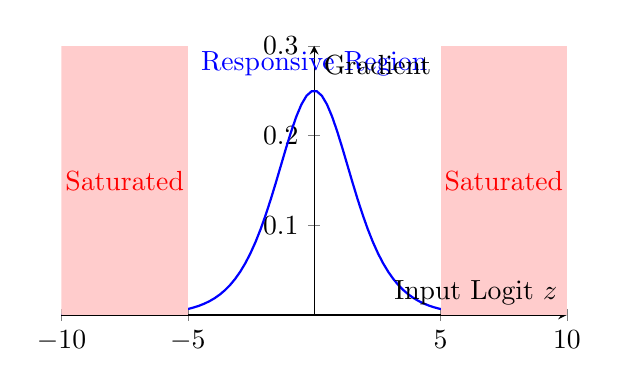
\begin{tikzpicture}
\begin{axis}[
width=8cm,
height=5cm,
xlabel={Input Logit $z$},
ylabel={Gradient},
domain=-10:10,
samples=100,
axis lines=middle,
ymin=0, ymax=0.3
]
% Derivative of sigmoid as proxy for gradient behavior
\addplot[blue, thick, domain=-10:10] {exp(-x)/((1+exp(-x))^2)};

% Saturation regions
\fill[red!20] (axis cs:5,0) rectangle (axis cs:10,0.3);
\fill[red!20] (axis cs:-10,0) rectangle (axis cs:-5,0.3);

\node[red] at (axis cs:7.5, 0.15) {Saturated};
\node[red] at (axis cs:-7.5, 0.15) {Saturated};
\node[blue] at (axis cs:0, 0.28) {Responsive Region};

\end{axis}
\end{tikzpicture}
\end{center}

\begin{center}
\textit{When inputs are large, softmax gradients vanish (illustrated here by the derivative of the related sigmoid function).}
\end{center}

When the inputs to the softmax have high variance, the distribution becomes very peaky (one element dominates). This pushes the function into regions where it is very flat (saturated). In these regions, the gradients are vanishingly small, which severely impedes learning.

\begin{tcolorbox}[colback=yellow!5!white, colframe=orange!50!black, title={The Scaling Solution (Vaswani et al., 2017)}]
To counteract the growth in variance, we introduce the scaling factor $\frac{1}{\sqrt{d_k}}$. This ensures the scores have a stable variance regardless of the dimensionality:

\begin{equation}
\text{Var}\left(\frac{q^T k}{\sqrt{d_k}}\right) = \frac{1}{d_k} \text{Var}(q^T k) = \frac{d_k}{d_k} = 1
\end{equation}

This keeps the inputs to the softmax within a ``responsive'' region, leading to healthier gradients.
\end{tcolorbox}

\subsection{The Final Formula: Scaled Dot-Product Attention (SDPA)}

Putting the learned projections and the scaling factor together, we arrive at the standard formula for Scaled Dot-Product Attention:

\begin{equation}
a(q, k) = \frac{(W_Q q)^T (W_K k)}{\sqrt{d_k}}
\end{equation}

We can express this efficiently in matrix form. Let $H\in\mathbb{R}^{T\times d_{\text{enc}}}$ be the matrix of encoder states. In cross-attention, the decoder state $s_t\in\mathbb{R}^{d_{\text{dec}}}$ acts as the query.

We define the projected Queries, Keys, and Values:
\begin{itemize}
\item $Q = s_t W_Q \in \mathbb{R}^{1\times d_k}$ (Projected query from decoder)
\item $K = HW_K \in \mathbb{R}^{T\times d_k}$ (Projected keys from encoder)
\item $V = HW_V \in \mathbb{R}^{T\times d_v}$ (Projected values from encoder)
\end{itemize}

The attention output (the context vector $c_t$) is computed as:

\begin{equation}
\text{Attention}(Q, K, V) = \text{softmax}\left(\frac{QK^T}{\sqrt{d_k}}\right)V
\end{equation}

This entire operation is composed of two large matrix multiplications ($QK^T$ and the subsequent multiplication by $V$), plus the scaled softmax. This is highly optimized on modern hardware.

\subsection{Common Implementation Pitfalls}

\begin{tcolorbox}[colback=red!5!white, colframe=red!50!black, title=Watch Out For These Mistakes!]
\textbf{1. Forgetting to scale by $\sqrt{d_k}$:}
Without scaling, training becomes unstable for larger $d_k$ values. The softmax saturates and gradients vanish.

\textbf{2. Wrong dimension for softmax:}
Always apply softmax over the \textit{keys} dimension (dim=-1 in the scores tensor). Applying it over queries would normalize the wrong axis.

\textbf{3. Masking with zeros instead of large negative values:}
Setting masked positions to 0 before softmax is wrong! After softmax, they would still contribute positive probability. Use $-10^9$ or \texttt{float('-inf')}.

\textbf{4. Inconsistent batch matrix multiplication:}
PyTorch's \texttt{bmm()} requires exactly 3D tensors: (batch, n, m). If you have 2D, use \texttt{mm()}. If you have 4D, reshape first.

\textbf{5. Not handling variable-length sequences:}
Always implement proper masking for padded sequences. Attending to padding tokens introduces noise and degrades performance.
\end{tcolorbox}

\subsection{Addressing the ``Missing Non-linearity'' in RNN+Attention}

We have established that dot-product attention is faster than additive attention because it replaces the non-linear MLP ($\tanh$) with a simple bilinear operation (dot product). This raises a critical question: Have we lost expressive power by removing the non-linearity in the scoring function?

While the dot-product attention mechanism itself is bilinear, it does not operate in a vacuum. It relies on the surrounding architecture to provide the rich, non-linear features that the attention mechanism then matches and pools.

\begin{tcolorbox}[colback=blue!5!white, colframe=blue!75!black, title=Non-linearity in the RNN Seq2Seq Architecture]
In the context of the Encoder-Decoder architecture we are studying, the non-linearity is provided by the underlying Recurrent Neural Networks (RNNs).

\begin{enumerate}
\item \textbf{Rich Input Representations}: The inputs to the attention mechanism---the encoder states $\{h_i\}$ and the decoder state $s_t$---are \textbf{not} raw embeddings. They are the outputs of deep, recurrent processing (e.g., LSTMs or GRUs).
\item \textbf{Recurrent Non-linearities}: RNN cells contain explicit non-linear activation functions (sigmoid for gates, $\tanh$ for cell states/outputs). These functions are applied iteratively at every time step.
\item \textbf{Complex Feature Extraction}: This iterative, non-linear processing allows the hidden states to encode complex syntactic and semantic information. The RNNs effectively perform the non-linear feature lifting (the $\phi$ in our Kernel view).
\end{enumerate}

\textbf{The Role of Attention:}
The attention mechanism operates on a feature space that has already been non-linearly transformed by the RNNs. Because these features are already rich and expressive, the simple, linear projections ($W_Q, W_K$) are sufficient to align the query and keys effectively. The attention mechanism's job is selection and combination, not complex feature extraction.

\textbf{Contrast with Transformers (A Preview):}
Next lecture, we will introduce the Transformer architecture, which removes the RNNs entirely. Without the inherent non-linearity of the RNNs, the Transformer must introduce an explicit non-linear component between attention layers---the Positionwise Feed-Forward Network (FFN)---to provide the necessary expressive power.
\end{tcolorbox}

\subsection{Comparison: The Evolution Summarized}

We can now summarize the trade-offs between the two primary learned attention mechanisms:

\begin{center}
\begin{tabular}{|l|p{5cm}|p{5cm}|}
\hline
\textbf{Aspect} & \textbf{Additive (Bahdanau)} & \textbf{Scaled Dot-Product (Vaswani)} \\
\hline
Scoring Function & $\bm{v}^T \tanh(W_q q + W_k k)$ & $\frac{(W_Q q)^T (W_K k)}{\sqrt{d_k}}$ \\
\hline
Interaction & Non-linear (via $\tanh$ MLP) & Bilinear (dot product) \\
\hline
Expressiveness & High in isolation & Relies on underlying architecture (RNN/FFN) for non-linearity \\
\hline
Efficiency (Hardware) & Slower; Memory-bound due to broadcasting and elementwise ops & Faster; Compute-bound (optimized GEMM); Highly scalable on GPUs/TPUs \\
\hline
Dimensionality & Flexible ($d_q$ need not equal $d_k$) & Requires $d_q = d_k$ for the dot product \\
\hline
Key Insight & Learn the similarity function (MLP) & Learn the feature space (projections) \\
\hline
\end{tabular}
\end{center}



\subsection{Implementation}

\begin{lstlisting}[language=Python, caption=Scaled Dot-Product Attention]
class ScaledDotProductAttention(nn.Module):
    def __init__(self, dropout=0.0):
        super().__init__()
        self.dropout = nn.Dropout(dropout)
    
    def forward(self, queries, keys, values, valid_lens=None):
        """
        queries: (batch_size, num_queries, d_k)
        keys: (batch_size, num_keys, d_k)
        values: (batch_size, num_keys, d_v)
        """
        d_k = queries.shape[-1]
        
        # Compute scores: (b, num_q, d_k) @ (b, d_k, num_k)
        # Result: (b, num_q, num_k)
        scores = torch.bmm(queries, keys.transpose(1, 2)) / math.sqrt(d_k)
        # ^^ IMPROVEMENT: Use math.sqrt(d_k) instead of creating a tensor
        
        # Apply masked softmax
        attention_weights = masked_softmax(scores, valid_lens)
        
        # Weighted sum: (b, num_q, num_k) @ (b, num_k, d_v)
        # Result: (b, num_q, d_v)
        return torch.bmm(self.dropout(attention_weights), values)
\end{lstlisting}

\section{Practical Implementation: Batching and Masking}

\subsection{Batch Processing}

In practice, we process multiple examples simultaneously. Following PyTorch conventions:

\begin{tcolorbox}[colback=yellow!5!white, colframe=orange!50!black, title=Batch Dimensions]
\begin{itemize}
    \item $b$ = batch size
    \item $T_{\text{enc}}$ = encoder sequence length
    \item $T_{\text{dec}}$ = decoder sequence length (number of queries)
    \item $d_{\text{enc}}, d_{\text{dec}}, d_k, d_v$ = various feature dimensions
\end{itemize}

Tensor shapes for cross-attention:
\begin{align}
\text{Queries (from decoder)} &: (b, T_{\text{dec}}, d_{\text{dec}}) \\
\text{Keys (from encoder)} &: (b, T_{\text{enc}}, d_{\text{enc}}) \\
\text{Values (from encoder)} &: (b, T_{\text{enc}}, d_{\text{enc}}) \\
\text{Output context vectors} &: (b, T_{\text{dec}}, d_v)
\end{align}
\end{tcolorbox}

PyTorch's batch matrix multiplication follows:
\begin{equation}
(b, n, m) \otimes (b, m, p) \rightarrow (b, n, p)
\end{equation}

\subsection{Masked Softmax: Handling Variable Lengths}

Real sequences have different lengths. We pad shorter ones to a common length, but must prevent the model from attending to padding tokens.

\begin{lstlisting}[language=Python, caption=Masked Softmax for Padding]
def masked_softmax(scores, valid_lens=None):
    """
    Apply softmax with optional masking for padding.
    
    scores: (batch_size, num_queries, num_keys)
    valid_lens: (batch_size,) - number of valid encoder positions
                for each example
    """
    if valid_lens is None:
        return F.softmax(scores, dim=-1)
    
    shape = scores.shape
    # Expand valid_lens to match scores shape
    if valid_lens.dim() == 1:
        valid_lens = valid_lens.view(-1, 1, 1)
        valid_lens = valid_lens.repeat(1, shape[1], 1)
    else:
        valid_lens = valid_lens.view(shape[0], shape[1], 1)
    
    # Create mask: True for valid positions
    mask = torch.arange(shape[-1], device=scores.device)
    mask = mask.view(1, 1, -1).repeat(shape[0], shape[1], 1)
    mask = mask < valid_lens
    
    # Set invalid positions to large negative value
    scores = scores.masked_fill(~mask, -1e9)
    
    return F.softmax(scores, dim=-1)
\end{lstlisting}

\begin{tcolorbox}[colback=red!5!white, colframe=red!50!black, title=Important: No Causal Mask in Cross-Attention]
In decoder \textbf{cross-attention}, we do NOT use a causal mask. The decoder can attend to all encoder positions---there is no notion of ``future'' in the source sentence.

\textbf{Why?} The entire source sentence is available before we begin decoding. When translating ``Le chat noir'' to ``The black cat'', all three French words exist simultaneously. The decoder can freely look at any part of the source.

\textbf{Causal masking} (preventing attention to future positions) is only used for decoder \textbf{self-attention}, where we must prevent position $t$ from seeing positions $t+1, t+2, \ldots$ during training. We will cover this in the next lecture.
\end{tcolorbox}

\paragraph{Numerical Stability Considerations: Choosing the Right Mask Value}

When masking, we set invalid positions to a large negative value (we use $-10^9$). Why this specific choice? Let us understand the tradeoffs.

\textbf{What happens in softmax:}
Recall that softmax computes $\text{softmax}(z_i) = \frac{\exp(z_i)}{\sum_j \exp(z_j)}$. For a masked position to receive near-zero probability, we need $\exp(z_{\text{masked}})$ to be negligible compared to $\exp(z_{\text{valid}})$.

\textbf{Concrete example:}
Suppose we have scores $[2.5, 3.1, z_{\text{mask}}]$ where the third position is padding:

\begin{center}
\begin{tabular}{|l|c|c|c|c|}
\hline
\textbf{Mask Value} & $\exp(2.5)$ & $\exp(3.1)$ & $\exp(z_{\text{mask}})$ & \textbf{Probability on Padding} \\
\hline
$z_{\text{mask}} = -10$ & 12.18 & 22.20 & $4.5 \times 10^{-5}$ & $\approx 0.0001$ (too large!) \\
$z_{\text{mask}} = -10^9$ & 12.18 & 22.20 & $\approx 0$ & $\approx 0$ (good) \\
$z_{\text{mask}} = -10^{20}$ & 12.18 & 22.20 & underflow $\rightarrow$ 0 & 0 (but risky) \\
$z_{\text{mask}} = -\infty$ & 12.18 & 22.20 & 0 & 0 (perfect, but...) \\
\hline
\end{tabular}
\end{center}

\textbf{The tradeoffs:}

\begin{itemize}
    \item \textbf{Too small in magnitude (e.g., $-10$):} After $\exp(-10) \approx 0.000045$, the masked position still receives non-negligible probability. The model incorrectly attends to padding!
    
    \item \textbf{Too large in magnitude (e.g., $-10^{20}$):} In theory fine, but risks numerical issues. When computing $\exp(-10^{20})$ in finite precision, you might trigger underflow warnings or unstable gradients during backpropagation.
    
    \item \textbf{Exactly $-\infty$:} Mathematically perfect---$\exp(-\infty) = 0$. However, if \textit{all} positions are masked (edge case), you get $\frac{0}{0} = \texttt{NaN}$, which crashes training. Also, $\texttt{-inf} - \texttt{-inf}$ is undefined and can cause \texttt{NaN} gradients.
    
    \item \textbf{The sweet spot ($-10^9$):} Large enough that $\exp(-10^9)$ is effectively zero (probability $< 10^{-400}$), but small enough to avoid numerical pathologies.
\end{itemize}

\begin{tcolorbox}[colback=yellow!5!white, colframe=orange!50!black, title=Mixed-Precision Training (FP16/BF16)]
When using 16-bit floating point:
\begin{itemize}
    \item \textbf{FP16 range:} approximately $\pm 65,504$ (much smaller than FP32's $\pm 10^{38}$)
    \item Using $-10^9$ would overflow to $-\infty$ in FP16!
    \item \textbf{Solution:} Use \texttt{-65504} (or \texttt{torch.finfo(torch.float16).min}) as the mask value
    \item \textbf{BF16:} Has same exponent range as FP32, so $-10^9$ works fine
\end{itemize}

Modern frameworks (PyTorch, JAX) handle this automatically when you use their masking utilities.
\end{tcolorbox}

\textbf{Practical recommendation:}
Use $-10^9$ for FP32 training, and let your framework's masking utilities handle precision-specific values automatically (e.g., PyTorch's \texttt{torch.nn.functional.scaled\_dot\_product\_attention} with \texttt{attn\_mask}).
\subsection{Complete Cross-Attention Layer}

\begin{lstlisting}[language=Python, caption=Complete Cross-Attention for Decoder]
class DecoderCrossAttention(nn.Module):
    def __init__(self, d_dec, d_enc, d_k, d_v, dropout=0.1):
        super().__init__()
        self.W_q = nn.Linear(d_dec, d_k, bias=False)
        self.W_k = nn.Linear(d_enc, d_k, bias=False)
        self.W_v = nn.Linear(d_enc, d_v, bias=False)
        self.attention = ScaledDotProductAttention(dropout)
        
    def forward(self, decoder_state, encoder_memory, valid_lens=None):
        """
        decoder_state: (batch, T_dec, d_dec)
        encoder_memory: (batch, T_enc, d_enc)
        valid_lens: (batch,) - valid encoder sequence lengths
        
        Returns: (batch, T_dec, d_v)
        """
        # Project to query/key/value spaces
        Q = self.W_q(decoder_state)      # (b, T_dec, d_k)
        K = self.W_k(encoder_memory)     # (b, T_enc, d_k)
        V = self.W_v(encoder_memory)     # (b, T_enc, d_v)
        
        # Compute attention
        context = self.attention(Q, K, V, valid_lens)
        return context  # (b, T_dec, d_v)
\end{lstlisting}

\section{Multi-Head Attention: Multiple Perspectives}

\subsection{Why One Head Is Not Enough}

A single attention mechanism learns one specific notion of similarity. However, language involves multiple simultaneous relationships:

\begin{itemize}
    \item \textbf{Syntactic}: subject-verb agreement, dependencies
    \item \textbf{Semantic}: agent, patient, instrument roles
    \item \textbf{Referential}: pronoun resolution, coreference
    \item \textbf{Discourse}: topic continuity, paragraph structure
    \item \textbf{Positional}: local context, adjacent words
\end{itemize}

One similarity function cannot capture all these patterns simultaneously.

\begin{tcolorbox}[colback=blue!5!white, colframe=blue!50!black, title=Looking Ahead: MHA's Expanding Role]
In our current RNN architecture, the recurrent connection provides strong inductive biases about sequence order, locality (nearby words are related), and syntactic structure (handled by the gating mechanisms). 

If we were to remove the RNN entirely (as we will next lecture), the attention mechanism must capture all these diverse relationships on its own. Multi-Head Attention provides the capacity and flexibility for the model to learn these patterns directly from the data.
\end{tcolorbox}

% \subsection{The Multi-Head Solution}

% \textbf{Multi-Head Attention} learns $h$ independent attention functions in parallel, each discovering different types of relationships.

% Instead of one set of $(W_Q, W_K, W_V)$, we learn $h$ sets:

% \begin{equation}
% \text{head}_i = \text{Attention}(QW_Q^i, KW_K^i, VW_V^i)
% \end{equation}

% The outputs are concatenated and projected:

% \begin{equation}
% \text{MultiHead}(Q, K, V) = \text{Concat}(\text{head}_1, \ldots, \text{head}_h)W_O
% \end{equation}

% \begin{figure}[h]
% \centering
% \begin{tikzpicture}[scale=0.8]
%     % Input
%     \node[draw, rectangle, minimum width=2cm, minimum height=0.8cm, fill=blue!20] 
%         (input) at (0, 0) {$Q, K, V$};
    
%     % Heads
%     \foreach \i in {1,2,3} {
%         \node[draw, rectangle, minimum width=1.5cm, minimum height=1.2cm, 
%               fill=green!20] (head\i) at (3*\i - 1.5, 2) {Head $\i$};
%         \draw[->, thick] (input) -- (head\i);
%     }
    
%     % Concat
%     \node[draw, rectangle, minimum width=2cm, minimum height=0.8cm, 
%           fill=yellow!20] (concat) at (4.5, 4) {Concat};
    
%     \foreach \i in {1,2,3} {
%         \draw[->, thick] (head\i) -- (concat);
%     }
    
%     % Output projection
%     \node[draw, rectangle, minimum width=2cm, minimum height=0.8cm, 
%           fill=orange!20] (output) at (4.5, 5.5) {$W_O$};
%     \draw[->, thick] (concat) -- (output);
    
%     \node[above] at (output.north) {Output};
% \end{tikzpicture}
% \caption{Multi-head attention: parallel attention mechanisms learning different patterns}
% \end{figure}

% \subsection{Implementation}

% \begin{lstlisting}[language=Python, caption=Multi-Head Cross-Attention]
% class MultiHeadCrossAttention(nn.Module):
%     def __init__(self, d_dec, d_enc, d_model, num_heads, dropout=0.1):
%         super().__init__()
%         assert d_model % num_heads == 0
        
%         self.d_model = d_model
%         self.num_heads = num_heads
%         self.d_k = d_model // num_heads
        
%         # Projections for all heads (combined)
%         self.W_q = nn.Linear(d_dec, d_model, bias=False)
%         self.W_k = nn.Linear(d_enc, d_model, bias=False)
%         self.W_v = nn.Linear(d_enc, d_model, bias=False)
%         self.W_o = nn.Linear(d_model, d_model, bias=False)
        
%         self.attention = ScaledDotProductAttention(dropout)
        
%     def forward(self, decoder_state, encoder_memory, valid_lens=None):
%         """
%         decoder_state: (batch, T_dec, d_dec)
%         encoder_memory: (batch, T_enc, d_enc)
%         """
%         batch_size = decoder_state.shape[0]
        
%         # Linear projections and split into heads
%         # (b, T, d_model) -> (b, T, num_heads, d_k) -> (b, num_heads, T, d_k)
%         Q = self.W_q(decoder_state).view(
%             batch_size, -1, self.num_heads, self.d_k
%         ).transpose(1, 2)
        
%         K = self.W_k(encoder_memory).view(
%             batch_size, -1, self.num_heads, self.d_k
%         ).transpose(1, 2)
        
%         V = self.W_v(encoder_memory).view(
%             batch_size, -1, self.num_heads, self.d_k
%         ).transpose(1, 2)
        
%         # Reshape for batch processing: (b*num_heads, T, d_k)
%         Q = Q.reshape(batch_size * self.num_heads, -1, self.d_k)
%         K = K.reshape(batch_size * self.num_heads, -1, self.d_k)
%         V = V.reshape(batch_size * self.num_heads, -1, self.d_k)
        
%         # Repeat valid_lens for each head
%         if valid_lens is not None:
%             valid_lens = valid_lens.repeat_interleave(self.num_heads)
        
%         # Apply attention
%         attn_output = self.attention(Q, K, V, valid_lens)
        
%         # Reshape and concatenate heads
%         # (b*num_heads, T_dec, d_k) -> (b, num_heads, T_dec, d_k)
%         attn_output = attn_output.reshape(
%             batch_size, self.num_heads, -1, self.d_k
%         )
%         # (b, num_heads, T_dec, d_k) -> (b, T_dec, d_model)
%         attn_output = attn_output.transpose(1, 2).contiguous().reshape(
%             batch_size, -1, self.d_model
%         )
        
%         # Output projection
%         return self.W_o(attn_output)
% \end{lstlisting}


% \begin{tcolorbox}[colback=yellow!5!white, colframe=orange!50!black, title=Why .contiguous()?]
% After \texttt{transpose()}, the tensor's memory layout is no longer contiguous (elements are not stored sequentially in memory). The \texttt{.reshape()} operation requires contiguous memory, so we call \texttt{.contiguous()} to create a contiguous copy. 

% This is a PyTorch implementation detail: operations like \texttt{transpose()} create a view with different strides but don't physically rearrange memory. \texttt{reshape()} needs the data laid out sequentially.
% \end{tcolorbox}

% \begin{tcolorbox}[colback=blue!5!white, colframe=blue!75!black, title=Connection to PyTorch's Built-in Implementation]
% PyTorch provides \texttt{nn.MultiheadAttention}, which implements the same mechanism with additional optimizations:

% \begin{lstlisting}[language=Python]
% mha = nn.MultiheadAttention(
%     embed_dim=512,    # d_model
%     num_heads=8,
%     dropout=0.1,
%     batch_first=True  # Use (batch, seq, feature) order
% )

% # For cross-attention:
% output, attn_weights = mha(
%     query=decoder_state,      # (batch, T_dec, d_model)
%     key=encoder_memory,       # (batch, T_enc, d_model)
%     value=encoder_memory,     # (batch, T_enc, d_model)
%     key_padding_mask=mask     # (batch, T_enc) - True for padding
% )
% \end{lstlisting}

% Our implementation above teaches the concepts. In practice, use PyTorch's optimized version, which includes:
% \begin{itemize}
%     \item Fused kernels for better performance
%     \item Support for key/value caching (important for inference)
%     \item Optional bias terms
%     \item Flexible masking options
% \end{itemize}
% \end{tcolorbox}

% \subsection{What Do Different Heads Learn?}

% Empirical studies (Voita et al., 2019) analyzing trained models show:
% \begin{itemize}
%     \item Some heads track \textbf{syntactic structure} (e.g., attending to the subject when processing a verb)
%     \item Some heads capture \textbf{positional patterns} (e.g., attending to adjacent words)
%     \item Some heads focus on \textbf{rare words} or named entities
%     \item Some heads learn \textbf{semantic roles} (agent, patient, etc.)
%     \item Interestingly, some heads learn redundant patterns and can be pruned without performance loss
% \end{itemize}

\section{Where Cross-Attention Fits: The Attention-Augmented RNN Decoder Loop}

Let us see where cross-attention sits in the decoder's generation process. Crucially, in this architecture (pre-Transformer), the decoder is still an RNN, augmented by attention.

\begin{lstlisting}[language=Python, caption=Simplified Attention-Augmented RNN Decoder Step]
def decode_one_step(input_token, prev_decoder_state, encoder_memory, valid_lens):
    """
    One step of autoregressive decoding in an Attention-Augmented RNN.
    
    input_token: (batch, 1, d_emb) - embedding of the previously generated token (y_{t-1})
    prev_decoder_state: (batch, 1, d_dec) - previous RNN hidden state (s_{t-1})
    encoder_memory: (batch, T_enc, d_enc) - full encoder outputs (H)
    valid_lens: (batch,) - valid encoder lengths
    """
    # The exact mechanism varies (e.g., Bahdanau vs. Luong styles).
    # Here we follow the Bahdanau style:
    
    # 1. Cross-attention: Use the *previous* state s_{t-1} as the query 
    # to attend to encoder memory H.
    context = cross_attention(
        prev_decoder_state, encoder_memory, valid_lens
    )  # c_t
    
    # 2. RNN Update: Compute the new state s_t
    # The RNN cell combines the input token y_{t-1}, the previous state s_{t-1}, 
    # and the new context c_t.
    # s_t = RNN_dec(y_{t-1}, s_{t-1}, c_t)
    current_decoder_state = decoder_rnn_cell(
        input_token, prev_decoder_state, context
    ) 
    
    # 3. Project to vocabulary for next token prediction
    # Often the output projection uses a combination of s_t and c_t
    logits = output_projection(current_decoder_state, context) 
    
    return logits, current_decoder_state
\end{lstlisting}

At each step $t$ in the Attention-Augmented RNN decoder:
\begin{enumerate}
    \item The decoder uses its previous state $s_{t-1}$ as a query
    \item Cross-attention dynamically queries the encoder memory to compute $c_t$
    \item The RNN cell combines the input token, previous state, and context to compute the new state $s_t$
    \item The model predicts the next token using $s_t$ and $c_t$
\end{enumerate}

This dynamic lookup mechanism solves the bottleneck: when translating ``chat noir'' to ``black cat'', the decoder attends to ``noir'' when generating ``black'', then attends to ``chat'' when generating ``cat''.



\section{Summary: The Journey So Far}

\subsection{What We Learned Today}

\begin{enumerate}
    \item \textbf{The bottleneck problem}: A single context vector cannot capture long, complex sequences
    
    \item \textbf{RNN limitations}: Beyond bottleneck, sequential computation prevents parallelization
    
    \item \textbf{The solution}: Keep all encoder states as a memory bank, use dynamic lookup via cross-attention
    
    \item \textbf{The human analogy}: Translators work ``part by part'', not by memorizing everything
    
    \item \textbf{Architecture context}: We augment RNNs with attention, not replace them (yet)
    
    \item \textbf{The conceptual bridge}: Kernel regression shows attention is learned data pooling
    
    \item \textbf{The terminology mapping}: Query, keys, values, weights---each has clear meaning
    
    \item \textbf{Key vs. Value distinction}: Same vectors in basic attention, but distinct roles
    
    \item \textbf{The evolution}: From fixed kernels to additive attention to dot-product attention
    
    \item \textbf{The theory}: Two perspectives on dot products (feature spaces and distance expansion)
    
    \item \textbf{The scaling factor}: $\frac{1}{\sqrt{d_k}}$ maintains stable variance for effective training
    
    \item \textbf{Hardware efficiency}: Dot-product formulation enables BLAS optimization
    
    \item \textbf{Practical concerns}: Batching, padding masks, efficient implementation
    
    \item \textbf{Multiple perspectives}: Multi-head attention captures diverse relationships
    
    \item \textbf{Positional information}: Still relies on RNN recurrence for sequence order
\end{enumerate}

\subsection{The Transformation Chain}

\begin{center}
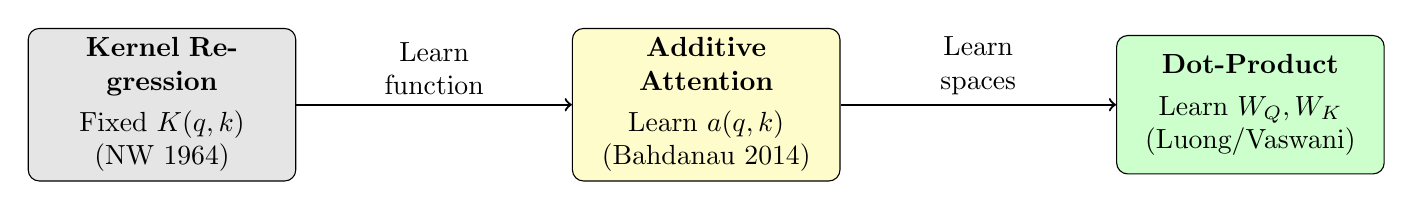
\begin{tikzpicture}[node distance=3.5cm, auto]
    \tikzstyle{block} = [rectangle, draw, text width=9em, text centered, 
                         rounded corners, minimum height=5em]

    \node [block, fill=gray!20] (kr) {
        \textbf{Kernel Regression}\\[0.3em]
        Fixed $K(q, k)$\\
        (NW 1964)
    };
    \node [block, fill=yellow!20, right=of kr] (add) {
        \textbf{Additive Attention}\\[0.3em]
        Learn $a(q, k)$\\
        (Bahdanau 2014)
    };
    \node [block, fill=green!20, right=of add] (dot) {
        \textbf{Dot-Product}\\[0.3em]
        Learn $W_Q, W_K$\\
        (Luong/Vaswani)
    };

    \draw[->, thick] (kr) -- node[align=center, above] {Learn\\function} (add);
    \draw[->, thick] (add) -- node[align=center, above] {Learn\\spaces} (dot);
\end{tikzpicture}
\end{center}

\section{Looking Ahead: The Leap to Self-Attention}

Today we focused on \textbf{cross-attention} integrated into an RNN-based Seq2Seq model. This approach---\textbf{Attention-Augmented RNNs}---solved the information bottleneck by allowing dynamic access to source information and was the state-of-the-art from 2015-2017.

However, as highlighted in Section 1, this architecture still suffers from the inherent limitations of recurrence:

\begin{enumerate}
    \item \textbf{The Sequential Bottleneck}: Training cannot be parallelized because RNNs process tokens one at a time.
    \item \textbf{Long-Range Dependencies}: Capturing very long-range dependencies \textit{within} the encoder (or decoder) itself remains difficult.
\end{enumerate}

The power lies in the generalized Query-Key-Value framework we developed. Crucially, this framework doesn't care where Q, K, and V come from. This leads to a radical idea: \textit{What if Q, K, and V all come from the \textbf{same} sequence? And what if we use this mechanism to replace recurrence entirely?}

\begin{tcolorbox}[colback=blue!5!white, colframe=blue!75!black, title=Preview: Self-Attention]
In \textbf{self-attention}, the queries, keys, and values all come from the \textit{same} sequence:

\begin{itemize}
    \item Each word can attend to every other word (including itself)
    \item We can capture long-range dependencies without recurrence
    \item We need \textbf{causal masking} for autoregressive generation (no peeking at future tokens)
    \item Positional encodings become essential (no RNN to track position)
    \item The entire sequence can be processed in parallel
\end{itemize}

This is the foundation of the Transformer architecture, which has revolutionized NLP and beyond.
\end{tcolorbox}

\subsection{The Big Questions for Next Time}

\begin{enumerate}
    \item If we remove recurrence entirely and use only attention, how do we model sequential order?
    \item How do we prevent the decoder from ``cheating'' by looking at future tokens?
    \item Can a model with no recurrence and no convolution really work?
    \item What enables Transformers to scale to billions of parameters?
    \item How does self-attention enable parallel computation across sequence positions within a training layer?
\end{enumerate}

\begin{tcolorbox}[colback=green!5!white, colframe=green!50!black, title=The Cliffhanger]
Cross-attention solved the encoder-decoder bottleneck. But the RNN architecture still limits us. What if attention is not just a helpful addition, but \textit{all} you need? What if we could build an entire model using only attention mechanisms, dispensing with recurrence entirely?

Next lecture: \textbf{Self-Attention and the Transformer Revolution}.
\end{tcolorbox}

\section{Exercises}

\begin{enumerate}
    \item \textbf{Concrete Example}: Take the French sentence ``Le chat noir dort sur le tapis rouge'' (The black cat sleeps on the red carpet). If you had to compress this into a single 512-dimensional vector for translation, what information might be lost? How would dynamic attention help?
    
    \item \textbf{Architecture Understanding}: Draw a diagram showing the flow of information in an attention-augmented RNN decoder for one decoding step. Clearly indicate where the RNN cell is, where cross-attention happens, and how they interact.
    
    \item \textbf{Derivation}: Starting from the Gaussian kernel $K(q, k) = \exp(-\|q - k\|^2 / 2h^2)$, carefully derive the equation $a(q, k) = q^T k - \frac{1}{2}\|q\|^2 - \frac{1}{2}\|k\|^2$ (taking $h=1$). Explain why the query-norm term cancels by softmax shift-invariance, and state the additional equal-key-norm assumption needed for the key-norm term to cancel.
    
    \item \textbf{Variance Analysis}: Generate random vectors $q, k \in \mathbb{R}^{d_k}$ with i.i.d. components from $\mathcal{N}(0, 1)$ for $d_k = 16, 64, 256$. Empirically verify that $\text{Var}(q^T k) = d_k$ and $\text{Var}(q^T k / \sqrt{d_k}) = 1$.
    
    \item \textbf{Implementation Comparison}: Implement both additive and scaled dot-product attention from scratch. Compare their runtime for $T_{\text{enc}} = 50, 100, 200$ and $d_k = 64, 128, 256$. Plot the results and explain the difference.
    
    \item \textbf{Masking Practice}: Create a batch of 4 sequences with encoder lengths $[7, 10, 8, 12]$, padded to length 12. Implement padding masks and verify that:
    \begin{itemize}
        \item Attention weights sum to 1.0 only over valid positions
        \item Padding positions receive near-zero weight
    \end{itemize}
    
    % \item \textbf{Multi-Head Visualization}: 
    % \begin{itemize}
    %     \item \textit{Option A (Recommended):} Use a pre-trained translation model (e.g., from HuggingFace Transformers). Extract and visualize attention patterns from each of the 4 heads for a sample input sentence.
    %     \item \textit{Option B (Advanced):} Train a small 2-layer seq2seq model with 4-head attention on a toy dataset (e.g., copy task or number sorting). Training code template provided in course repository.
    % \end{itemize}
    % Do different heads learn different patterns? Can you identify what each head focuses on?
    
    \item \textbf{Feature Space Analysis}: For a trained attention layer, compute the Gram matrices $Q Q^T$ and $K K^T$. What do these matrices tell you about the learned feature spaces?
    
    \item \textbf{Key vs. Value}: In the basic cross-attention we discussed, keys and values are the same ($k_i = v_i = h_i$). Propose a modification where keys and values are different projections. What might be the advantage?
    
    \item \textbf{Design Challenge}: Propose a hybrid attention mechanism that:
    \begin{itemize}
        \item Uses additive attention for the first layer (more flexible)
        \item Switches to dot-product for subsequent layers (more efficient)
        \item Justify your design choices
    \end{itemize}
\end{enumerate}

\section{Further Reading}

\subsection{Foundational Papers}

\begin{itemize}
    \item Nadaraya, E. A. (1964). On Estimating Regression. \textit{Theory of Probability and Its Applications}.
    \item Watson, G. S. (1964). Smooth Regression Analysis. \textit{Sankhya: The Indian Journal of Statistics}.
    \item Bahdanau, D., Cho, K., \& Bengio, Y. (2015). Neural Machine Translation by Jointly Learning to Align and Translate. \textit{ICLR}.
    \item Luong, M. T., Pham, H., \& Manning, C. D. (2015). Effective Approaches to Attention-based Neural Machine Translation. \textit{EMNLP}.
    \item Vaswani, A., et al. (2017). Attention Is All You Need. \textit{NeurIPS}.
\end{itemize}

\subsection{Analysis and Interpretation}

\begin{itemize}
    \item Voita, E., et al. (2019). Analyzing Multi-Head Self-Attention: Specialized Heads Do the Heavy Lifting, the Rest Can Be Pruned. \textit{ACL}.
    \item Michel, P., Levy, O., \& Neubig, G. (2019). Are Sixteen Heads Really Better than One? \textit{NeurIPS}.
\end{itemize}

\subsection{Textbooks}

\begin{itemize}
    \item Zhang, A., et al. (2023). \textit{Dive into Deep Learning}. Chapter 11: Attention Mechanisms and Transformers.
    \item Jurafsky, D., \& Martin, J. H. (2023). \textit{Speech and Language Processing} (3rd ed.). Chapter 10: Transformers and Large Language Models.
\end{itemize}

\end{document}
